% Informe complementario QA-E2E-20261003. La matriz detallada vive en auditoria-operativa-2026-10-03.md.
\documentclass[10pt,letterpaper]{article}
\usepackage[utf8]{inputenc}
\usepackage[T1]{fontenc}
\usepackage[spanish,es-nodecimaldot]{babel}
\usepackage[letterpaper,margin=1.9cm,headheight=14pt]{geometry}
\usepackage{xcolor,graphicx,tabularx,longtable,booktabs,array,float,hyperref,fancyhdr,caption}
\ifdefined\pdfinfoomitdate\pdfinfoomitdate=1\fi
\ifdefined\pdftrailerid\pdftrailerid{}\fi
\ifdefined\pdfsuppressptexinfo\pdfsuppressptexinfo=15\fi
\definecolor{azul}{HTML}{07579B}
\definecolor{verde}{HTML}{087359}
\definecolor{rojo}{HTML}{A03429}
\hypersetup{colorlinks=true,linkcolor=azul,pdftitle={Auditoria operativa BI IA 2026-10-03}}
\pagestyle{fancy}\fancyhf{}\lhead{Auditoría operativa BI + IA}\rhead{QA-E2E-20261003}\cfoot{\thepage}
\setlength{\parindent}{0pt}\setlength{\parskip}{0.45em}
\renewcommand{\arraystretch}{1.15}
\newcommand{\ok}{\textcolor{verde}{\textbf{Aprobado}}}
\newcommand{\pending}{\textcolor{rojo}{\textbf{Pendiente}}}
\begin{document}
\begin{titlepage}
\vspace*{1cm}{\color{azul}\rule{\textwidth}{3pt}}
\vspace{1.3cm}
{\Large Universidad de Guayaquil\\Facultad de Ciencias Matemáticas y Físicas\\Carrera de Software\par}
\vfill
{\Huge\bfseries Auditoría operativa del sistema BI asistido por IA\par}
\vspace{0.5cm}{\Large Casos funcionales, evidencia cuantitativa y límites semánticos\par}
\vspace{0.8cm}{\large AdventureWorks2022 y WideWorldImporters\par}
\vfill
\begin{tabularx}{\textwidth}{@{}>{\bfseries}p{0.28\textwidth}X@{}}
Código & QA-E2E-20261003\\
Fecha & 3 de octubre de 2026\\
Entorno & Docker Compose local, dos fuentes SQL Server\\
Rama & \texttt{fix/qa-operational-20261003}\\
Resultado & Ciclos AW \#98/\#14 y WWI \#114/\#15 completos; asesor previo con dos revisiones finales viables y reformulación aún limitada; roles sin sesión segregada\\
\end{tabularx}
\vspace{1cm}{\color{azul}\rule{\textwidth}{3pt}}
\end{titlepage}
\pagenumbering{arabic}

\section{Propósito y método}
La evaluación adoptó tres perspectivas complementarias. QA revisó navegación, aislamiento, recuperación y regresiones. El analista BI examinó granularidad, fórmulas, rutas y conciliación. La gerencia comercial distinguió pedidos registrados de facturas emitidas y exigió que el tablero declarase su alcance. Se recorrió la interfaz real y se contrastaron agregados con consultas de sólo lectura. No se enviaron filas ni credenciales a proveedores de IA.

\begin{table}[H]\centering
\caption{Inventario de metadatos por fuente}
\begin{tabular}{@{}lrrrrr@{}}\toprule
Fuente & Instantánea & Esquemas & Tablas & Columnas & Relaciones\\\midrule
AdventureWorks2022 & 2 & 6 & 71 & 482 & 90\\
WideWorldImporters & 3 & 4 & 48 & 546 & 98\\\bottomrule
\end{tabular}\end{table}

El catálogo de AdventureWorks conservó seis preguntas, incluidas dos añadidas por el analista; WideWorldImporters mostró cuatro. Se crearon los roles Analista BI y Gerente comercial sin usuarios asignados. El segundo recibió sólo consulta del tablero y de conexiones, más descarga de informes, después de autorización explícita. La prueba funcional con usuarios autenticados bajo esos roles sigue pendiente.

\section{Matriz de casos ejecutados}
\small
\begin{longtable}{@{}p{0.09\textwidth}p{0.46\textwidth}p{0.28\textwidth}p{0.10\textwidth}@{}}
\caption{Resultado observado frente al criterio de aceptación}\\\toprule
ID & Procedimiento y criterio & Observación & Estado\\\midrule\endfirsthead
\toprule ID & Procedimiento y criterio & Observación & Estado\\\midrule\endhead
QA-01 & Alternar fuente en Inicio y Explorador; no reutilizar contenido de otra página. & Se corrigió la excepción por respuesta de Roles tratada como metadatos. & \ok\\
QA-02 & Revisar catálogo separado y preservar preguntas de AW. & AW 6; WWI 4. No hubo contaminación cruzada. & \ok\\
QA-03 & Crear propuesta mensual AW y revisar promedio transaccional. & \#97 usó promedio de líneas; se descartó. \#98 usa ventas / documentos distintos. & \ok\\
QA-04 & Verificar, aprobar y materializar \#98. & 0 errores, 3 advertencias; ejecución \#14 con 121.317 filas origen y destino. & \ok\\
QA-05 & Filtrar 2014, explorar gráfico y preguntar Top 5 al copiloto. & 20,1 M; 11.761 pedidos; respuesta territorial con denominador explícito. & \ok\\
QA-06 & Exigir facturas en WWI y comparar con pedidos. & \#99 y \#100 eligieron pedidos; se bloquearon. \#114 usa líneas y fecha de factura. & \ok\\
QA-07 & Recuperar Claude tras JSON inválido. & Salida estructurada nativa y reintento acotado; la validación local se mantuvo. Groq 429; Gemini 400. & \ok\\
QA-08 & Rechazar KPI semánticamente engañosos. & \#113 confundió máximo de línea con producto líder y AVG de línea con promedio por cliente. Excluidos en \#114; regla bilingüe añadida. & \ok\\
QA-09 & Ejecutar y conciliar facturación WWI. & \#15: 228.265/228.265 filas, 70.510 facturas, 198.043.439,45 y promedio 2.808,73. & \ok\\
QA-10 & Filtrar 2015 y conversar con Claude. & 62.090.220,81 / 22.250 = 2.790,57; explicó factura, impuesto y no cobro. & \ok\\
QA-11 & Alternar \#15, \#13 y AW \#14. & Los tableros conservan fuente, expediente, indicadores y alcance separados. & \ok\\
QA-12 & Crear rol Gerente comercial sin asignarlo. & Tres permisos de consulta/descarga; prueba autenticada con ese rol pendiente. & \pending\\
\bottomrule\end{longtable}
\normalsize

\section{Conciliación y juicio de negocio}
En AdventureWorks, el origen contiene 121.317 líneas, 31.465 pedidos y 109.846.381,4250 de importe. El promedio correcto por pedido es 3.491,065673, mostrado como 3.491,07 en la ejecución \#14. El ETL cargó 121.317 filas, diferencia cero y cinco tablas. Se publicaron etiquetas españolas para tres grupos territoriales; se excluyeron códigos de país que no requerían traducción.

En WideWorldImporters, \texttt{Sales.OrderLines} contiene 231.412 líneas, 73.595 pedidos y 177.634.276,40 de valor calculado. \texttt{Sales.InvoiceLines} contiene 228.265 líneas, 70.510 facturas y 198.043.439,45 de \texttt{ExtendedPrice}; 172.261.341,20 corresponden a precio por cantidad y 25.782.098,25 a impuesto. Estos eventos y definiciones monetarias no son intercambiables. La ejecución histórica \#13 está conciliada con \emph{pedidos}. La nueva \#15 está conciliada con \emph{facturas emitidas}, no cobros, y conserva su propio esquema. El panel ofrece ambas sin cruzarlas. La divisa sigue descrita como moneda de origen porque no se verificó un código único.

\texttt{LastCostPrice} es el último costo registrado, no una prueba de costo histórico de cada factura. La versión WWI \#100 no fue aprobada; sus márgenes no deben presentarse como rentabilidad histórica sin esa evidencia.

\section{Evidencia visual de la ejecución}
\begin{figure}[H]\centering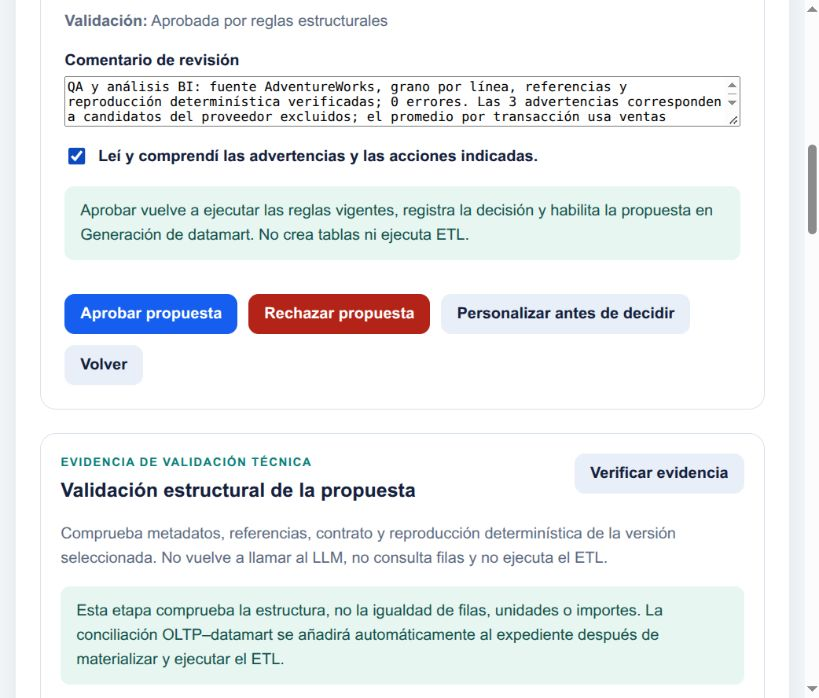
\includegraphics[width=0.85\textwidth]{evidencias/qa-20261003/08_validacion_aw.png}\caption{Propuesta AdventureWorks \#98: validación estructural antes de aprobación.}\end{figure}
\begin{figure}[H]\centering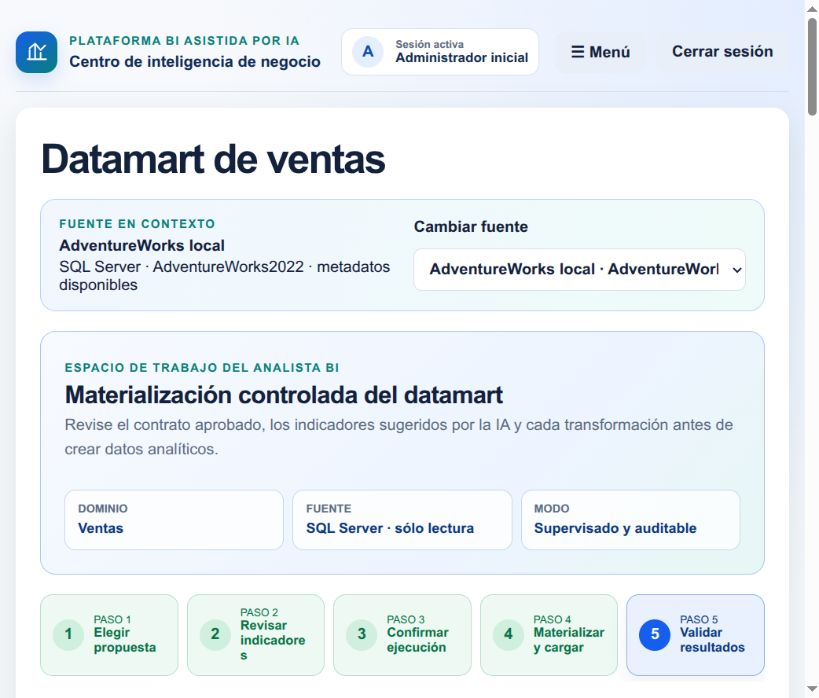
\includegraphics[width=0.85\textwidth]{evidencias/qa-20261003/12_conciliacion_aw.png}\caption{Ejecución \#14 en la etapa de validación; el contraste de filas figura en la sección 3.}\end{figure}
\begin{figure}[H]\centering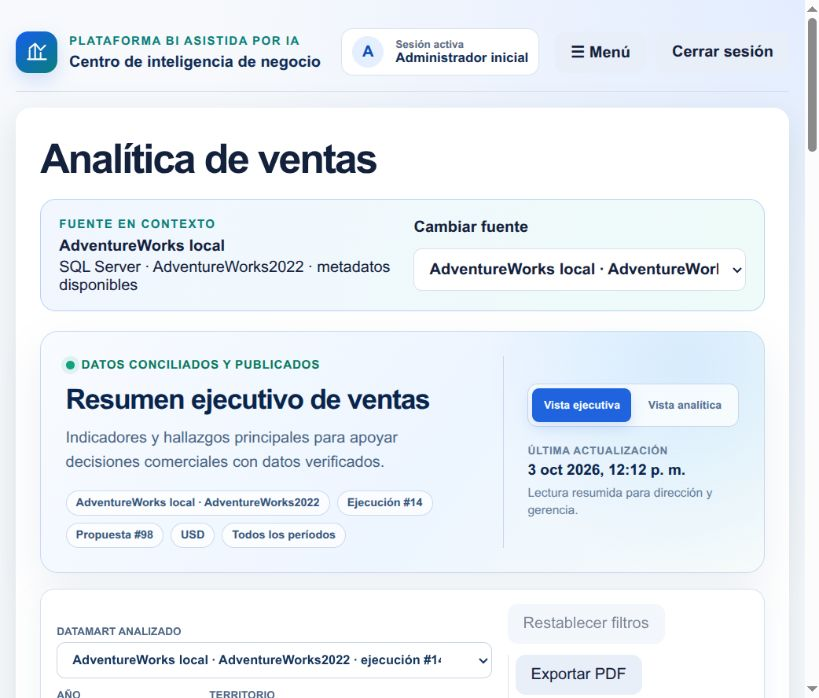
\includegraphics[width=0.85\textwidth]{evidencias/qa-20261003/14_dashboard_aw.png}\caption{Panel AdventureWorks posterior al ETL nuevo.}\end{figure}
\begin{figure}[H]\centering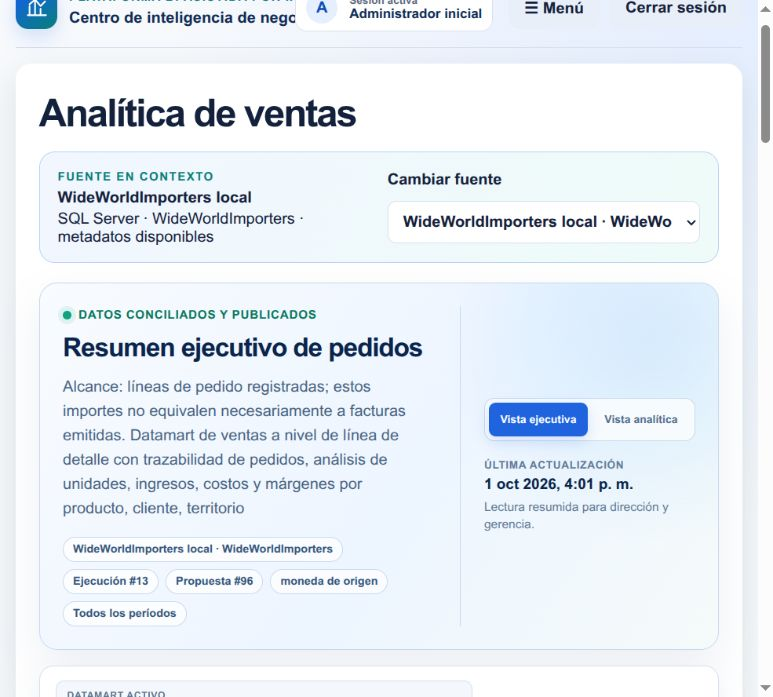
\includegraphics[width=0.85\textwidth]{evidencias/qa-20261003/24_dashboard_wwi_alcance.png}\caption{El expediente WWI histórico identifica su alcance: pedidos registrados, no facturas emitidas.}\end{figure}
\begin{figure}[H]\centering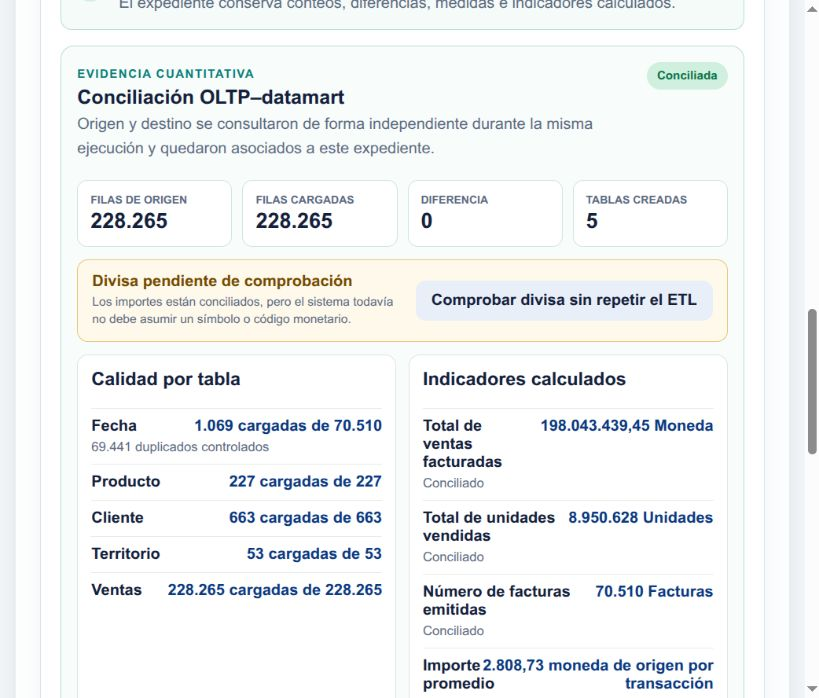
\includegraphics[width=0.85\textwidth]{evidencias/qa-20261003/31_wwi_facturas_etl15.png}\caption{Ejecución \#15: facturas conciliadas, 228.265 filas y seis indicadores.}\end{figure}
\begin{figure}[H]\centering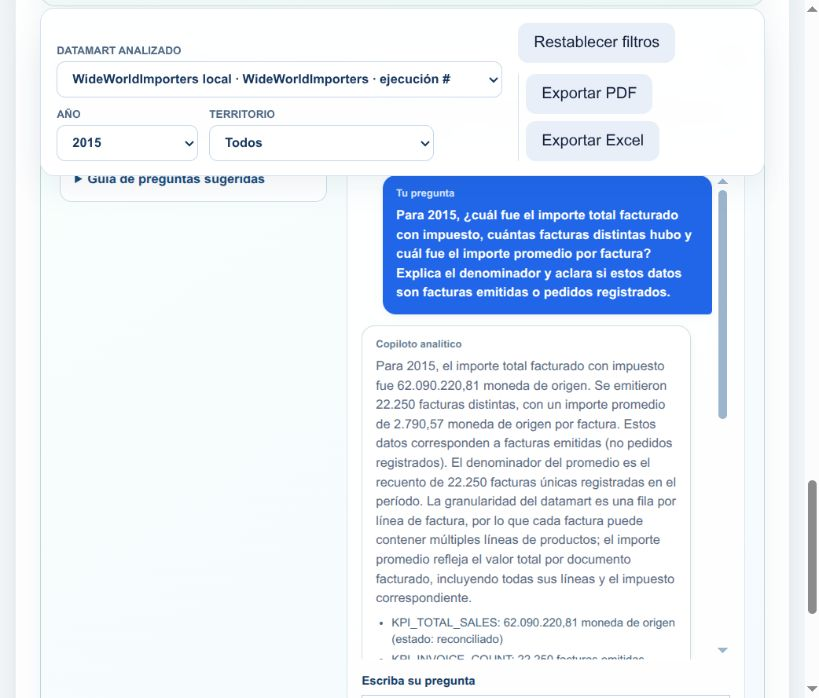
\includegraphics[width=0.85\textwidth]{evidencias/qa-20261003/32_wwi_facturas_copiloto2015.png}\caption{Claude interpreta 2015 con facturas distintas como denominador.}\end{figure}
\begin{figure}[H]\centering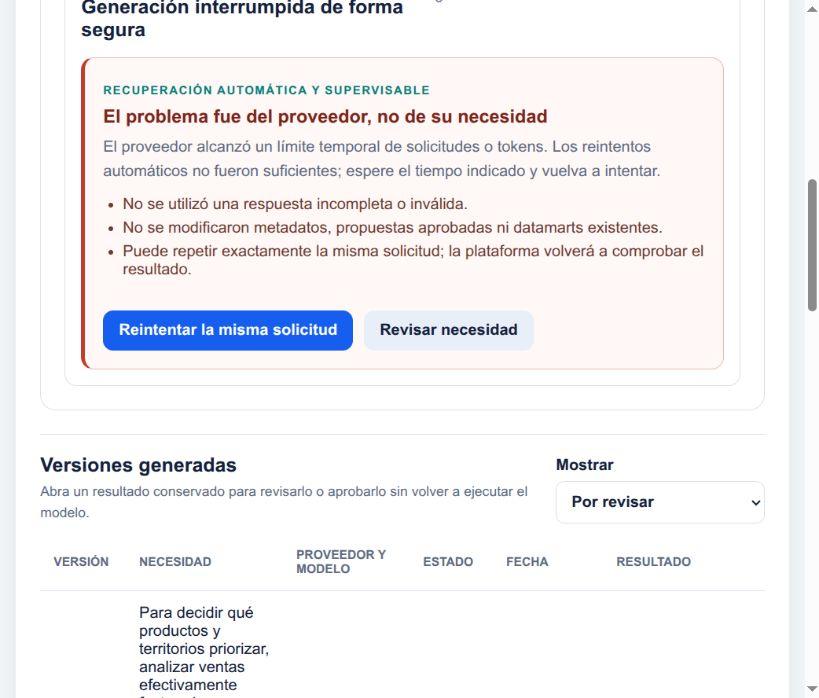
\includegraphics[width=0.85\textwidth]{evidencias/qa-20261003/23_groq_limite.png}\caption{Límite temporal de Groq: el asistente preserva la necesidad y no usa una respuesta incompleta.}\end{figure}

\clearpage
\section{Adenda: necesidades fundamentadas antes de la propuesta}

La revisión posterior encontró que la ayuda de redacción sólo enviaba una huella
de metadatos, no su estructura. Se añadió análisis previo de IA con tablas,
columnas, tipos, claves y relaciones permitidos; las referencias y rutas se
comprueban en el servidor. El analista puede escribir un objetivo o solicitar
sugerencias sin texto inicial. Debe elegir expresamente el texto y validar su
alcance antes de generar. La evaluación se guarda vinculada a fuente, instantánea,
actor y necesidad; cambiar el contexto obliga a validarla otra vez.

\small
\begin{longtable}{@{}p{0.13\textwidth}p{0.53\textwidth}p{0.23\textwidth}@{}}
\toprule Caso & Escenario y criterio & Resultado\\\midrule\endhead
NEED-01/03 & Costo desconectado, FK inversa o compuesta incompleta: no acreditar una derivación segura. & Aprobado en pruebas sintéticas.\\
NEED-02 & Importe textual o tipo desconocido: excluir o exigir revisión. & Aprobado.\\
NEED-04 & Factura aislada de pedidos: no declarar facturación comprobada. & Aprobado.\\
NEED-05 & Nombres españoles/ingleses y orden de tablas distinto: reglas generales estables. & Aprobado en fixtures.\\
NEED-06 & Referencia inventada y objetivo sin datos en salida IA simulada: no ocultar el límite. & Aprobado; no demuestra exhaustividad de un modelo real.\\
NEED-07/08 & Contexto con secretos/muestras y destino sin consentimiento: no transmitirlos. & Lista permitida y cero llamadas sin autorización.\\
NEED-09/10 & Objetivo vacío, adopción humana y respuesta tardía tras cambio de fuente. & 33 pruebas frontend aprobadas.\\
NEED-11 & Pantalla real WWI: sugerencias disponibles sólo tras consentimiento. & Observado sin llamada externa.\\
NEED-12 & Nuevas sugerencias y revisión real con Claude, AW y WWI. & Autorización recibida; resultados desglosados en la ampliación.\\
NEED-13/14 & Revisión--cobertura--propuesta; eliminar un margen, cambiar objetivo o destino. & El cálculo faltante bloquea; no se reutiliza alcance o consentimiento ajeno.\\
\bottomrule\end{longtable}
\normalsize

Se aplicó la migración aditiva \texttt{20261003\_19}, sin modificar propuestas
aprobadas o datamarts existentes. Las pruebas focalizadas de necesidades y servicio
aprobaron 83 casos y las del asesor 11. Los escenarios y criterios completos
están en la matriz QA-NEED del registro de auditoría.

\textbf{Interpretación:} respaldo estructural no garantiza filas completas,
significado financiero histórico o importes conciliados. La IA puede explicar
derivaciones y limitaciones; no reemplaza la aprobación humana ni las verificaciones
del modelo dimensional y ETL. Esta adenda no presenta los ciclos anteriores como
prueba de las nuevas rutas.

\begin{figure}[H]\centering
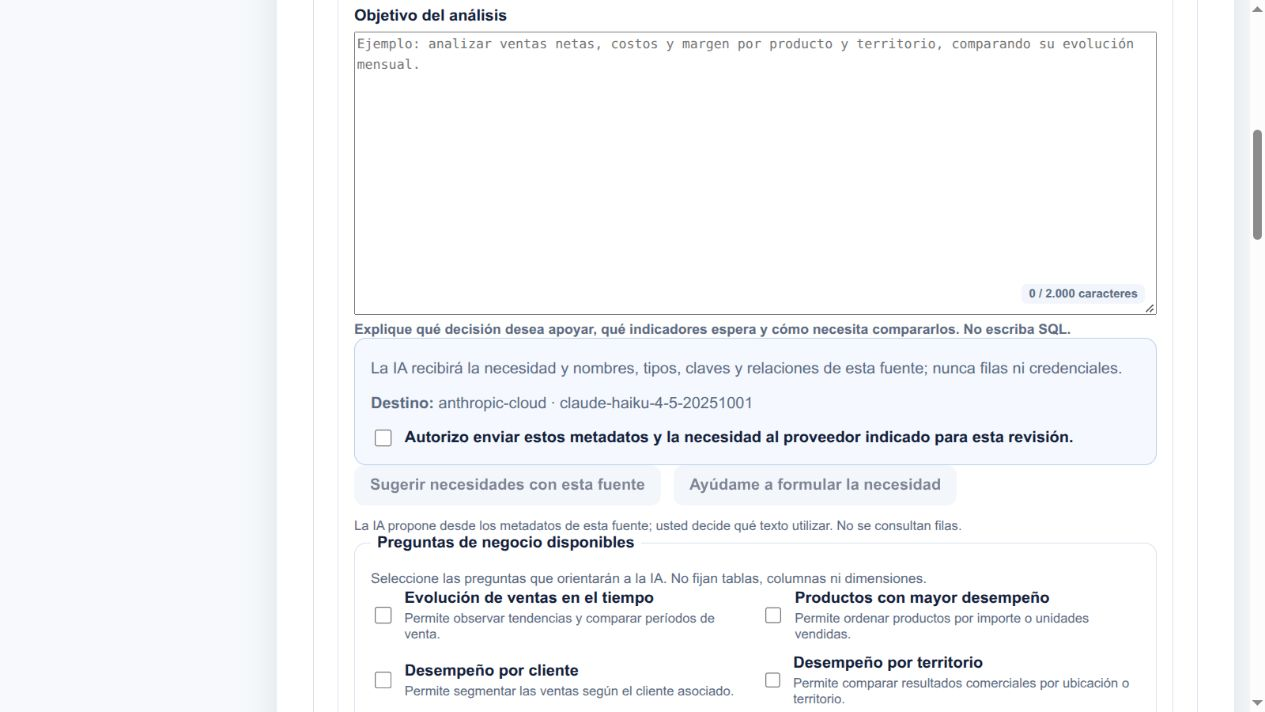
\includegraphics[width=0.92\textwidth]{evidencias/qa-20261003/33_necesidad_metadatos_consentimiento.png}
\caption{Paso Necesidad real, sin objetivo inicial ni consentimiento marcado. La imagen no representa una respuesta de Claude.}
\end{figure}

\section{Ampliación de la prueba real del asesor}

El usuario autorizó enviar a Claude únicamente necesidades de prueba y metadatos
estructurales de las dos fuentes. Se usó \texttt{claude-haiku-4-5-20251001} desde
la interfaz real. No se enviaron filas ni credenciales. Las versiones y ejecuciones
aprobadas se conservaron; estas pruebas no equivalen a ejecutar otro ETL.

\subsection{Incidentes observados}
Las primeras dos sugerencias de WideWorldImporters quedaron bloqueadas por
rutas, tipos o una capacidad sin validador. Una reformulación de facturación
también quedó no utilizable. El control local de la instantánea con ancla en
\texttt{Sales.InvoiceLines} verificó cinco requisitos directos: importe, cantidad,
fecha, producto y cliente. Las relaciones de los metadatos eran correctas.

Claude afirmó en una sugerencia bloqueada que \texttt{ExtendedPrice} excluía
impuestos. La estructura enviada no demuestra ese significado y la conciliación
previa de esta instalación acredita lo contrario. Se reforzó la instrucción general
de no inferir impuestos, moneda o costo histórico sólo de los nombres. Se conserva
la revisión humana: una explicación del modelo no es prueba financiera.

Una revisión que cambiaba el objetivo fue rechazada sin guardar una evaluación
de alcance distinto. La corrección automática entrega feedback verificable al
mismo destino consentido y mantiene un máximo de dos respuestas del asesor por
acción. Los reintentos de transporte del adaptador constituyen una política
separada; no se promete que toda respuesta probabilística sea aceptable.

La revisión inicial AW también confundió \texttt{UnitPrice} con costo. Se añadió
validación común de roles conocidos en español e inglés: precio no es costo, tasa
no es importe e identificador no es dinero. Un nombre desconocido exige
interpretación, no autoriza una equivalencia. \texttt{need-review-2} invalida la
reutilización de revisiones previas sin borrar historia ni retirar aprobaciones.

\subsection{Casos finales y resultados reproducibles}
La agrupación por mes quedó separada de las derivaciones aritméticas; una fecha
no se acepta como operando monetario. La corrección conserva el validador y entrega
orientación precisa al único reintento. La interfaz identifica el texto de la IA
como interpretación no ejecutable, no como fórmula financiera certificada.

\small
\begin{longtable}{@{}p{0.12\textwidth}p{0.42\textwidth}p{0.37\textwidth}@{}}
\toprule Caso & Procedimiento & Resultado observado\\\midrule\endhead
NEED-16 & WWI: pedir sugerencias sin objetivo y con periodicidad mensual. & Una utilizable y otra bloqueada; selección humana sin aprobar nada.\\
NEED-17 & AW: reformular importe y unidades mensuales por producto, con atributos. & Tras dos respuestas persistió una capacidad no soportada. No se adoptó; mantener el texto original funcionó.\\
NEED-18 & WWI: importe registrado por línea de factura, mensual, con trazabilidad. & Revisión \#5: 6 directos, 2 derivables, 4 advertencias, 0 no disponibles. Una respuesta. Aceptar límites habilitó continuar.\\
NEED-19 & AW: importe y unidades por producto, mensual, con identificador del pedido. & Revisión \#6: 11 directos, 1 derivable, 5 advertencias, 0 no disponibles. Una respuesta. Aceptar límites habilitó continuar.\\
NEED-20 & WWI: ventas mensuales e influencia de temperaturas externas por ciudad. & Clima no disponible; sensores de frío/vehículos no sustituyen meteorología. No se aceptó alcance parcial ni se habilitó generar.\\
NEED-21 & Cambiar texto y fuente; reanudar tras vencer la sesión. & Consentimiento reiniciado, autenticación requerida y revisión WWI no reutilizada en AW.\\
\bottomrule\end{longtable}
\normalsize

Los identificadores \#5 y \#6 son \emph{revisiones de necesidad}, no versiones de
propuesta ni expedientes ETL. Los conteos combinan reglas y revisión IA: no son
KPI únicos ni observaciones estadísticas independientes.
No se pulsó generar después de estos controles. Las
advertencias finales explican composición monetaria, fecha frente a cobro,
estados/población y cobertura de atributos; no se resolvieron inventando evidencia.
La matriz Markdown conserva los textos literales, preparación, incidencias y
archivos de evidencia. No se estima una tasa estadística de éxito porque se
introdujeron correcciones entre repeticiones.

\begin{figure}[H]\centering
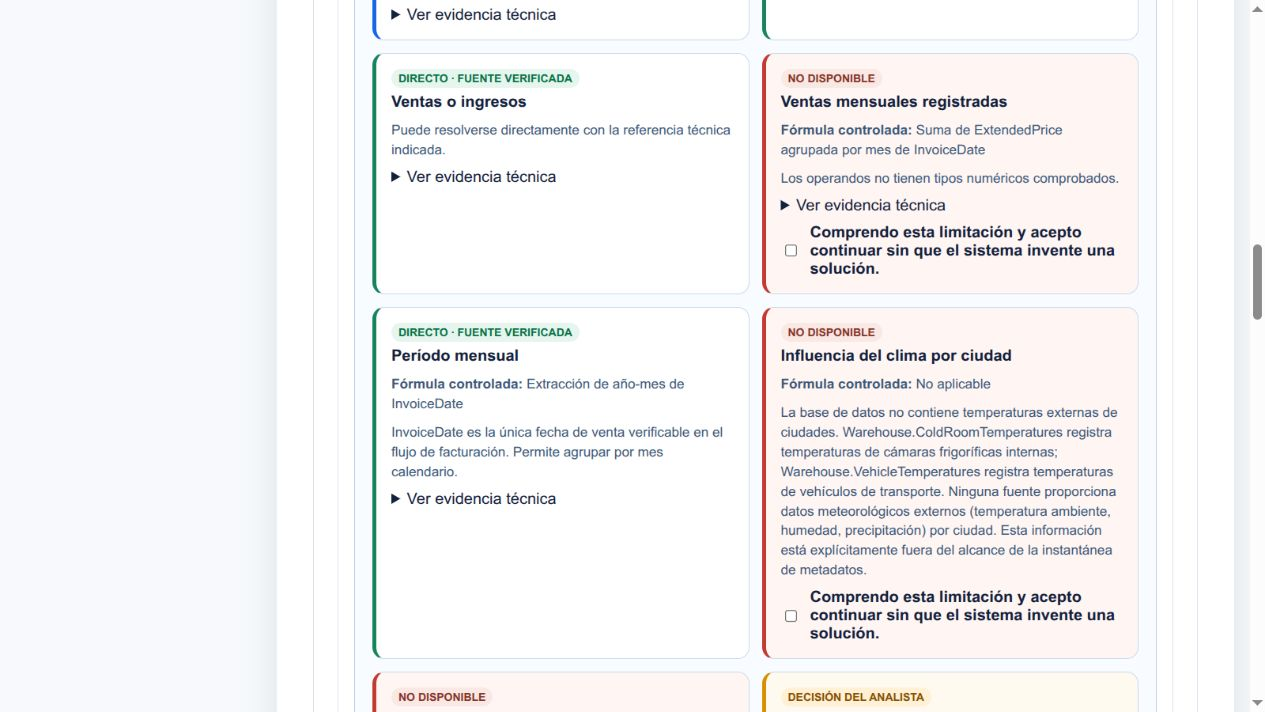
\includegraphics[width=0.92\textwidth]{evidencias/qa-20261003/35_necesidad_clima_no_disponible.png}
\caption{Caso negativo: clima externo ausente. La captura conserva además el fallo de agrupación temporal y las etiquetas anteriores, corregidos posteriormente; no representa la interfaz final.}
\end{figure}
\begin{figure}[H]\centering
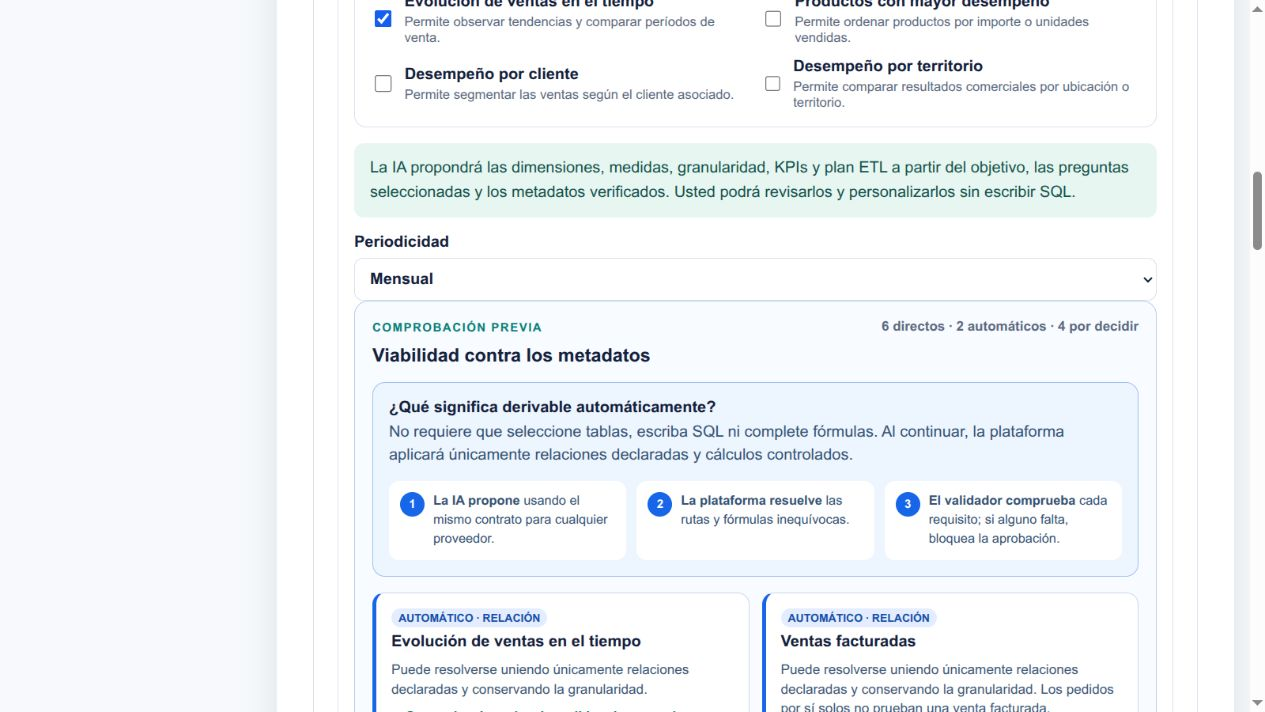
\includegraphics[width=0.92\textwidth]{evidencias/qa-20261003/36_necesidad_wwi_revision.png}
\caption{Revisión final WWI: seis requisitos directos, dos derivables y cuatro límites para decisión del analista.}
\end{figure}
\begin{figure}[H]\centering
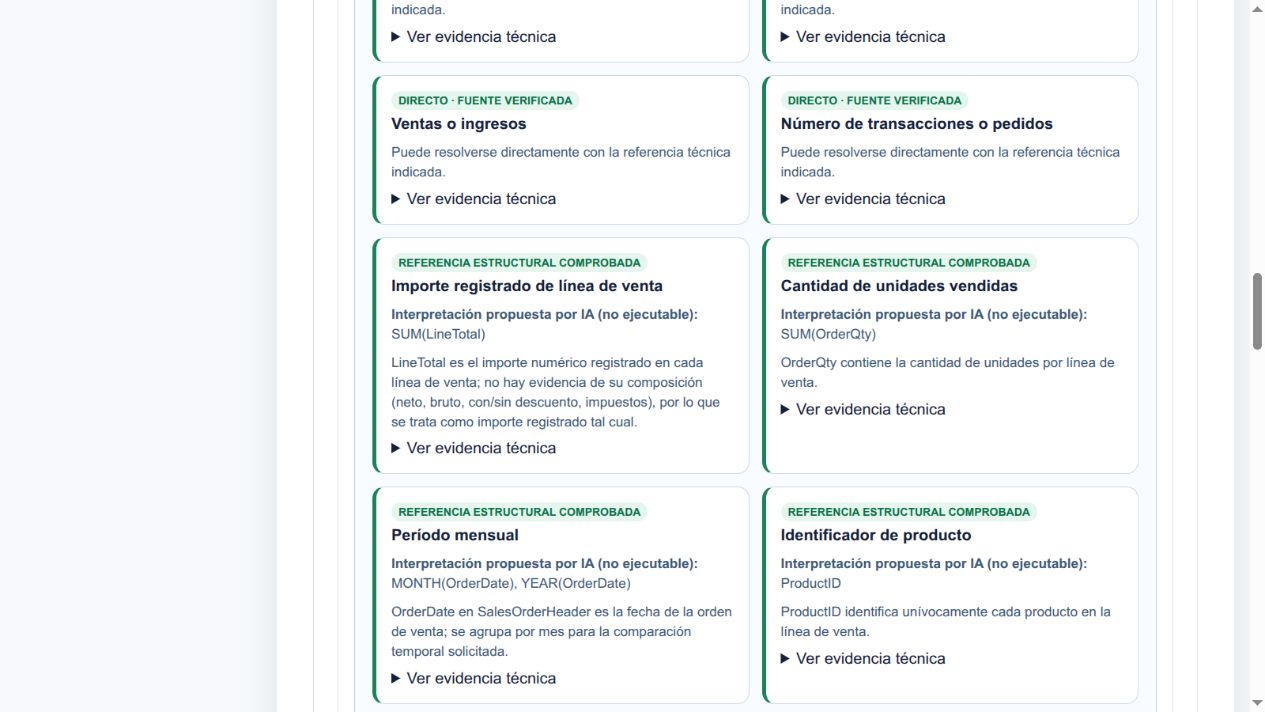
\includegraphics[width=0.92\textwidth]{evidencias/qa-20261003/38_necesidad_aw_interpretacion.png}
\caption{AW final: la interfaz distingue referencias estructurales de interpretaciones de IA no ejecutables.}
\end{figure}

\section{Cierre y límites para la tesis}
Los ciclos anteriores AW \#98/\#14 y WWI \#114/\#15 llegaron desde esquema y catálogo a propuesta, aprobación, ETL, conciliación, tablero y consulta del copiloto. El caso WWI detectó y corrigió una sustitución de pedidos por facturas, una afirmación del modelo que contradecía metadatos, una omisión de ventas en la cobertura y dos fórmulas de KPI con granularidad errónea. La recuperación de Claude no relajó el contrato común. Groq agotó cuota temporal y Gemini devolvió HTTP 400 en la prueba autorizada; Ollama no fue necesario. Tampoco se probó el inicio de sesión bajo los dos roles nuevos. La evidencia se limita a estas dos fuentes SQL Server y no demuestra universalidad para otros motores o dominios.

La ampliación del asesor previo termina con dos objetivos viables bajo revisión
humana y un negativo climático correctamente señalado. No repite los ETL. La
última reformulación AW siguió bloqueada, por lo que su aceptación es supervisada
y parcial: se puede conservar el texto del analista y validarlo. No se declara
que toda salida del proveedor será utilizable o financieramente correcta.

La regresión final \texttt{make test} aprobó 231 pruebas backend y 34 frontend,
con controles de formato, tipos, análisis estático y compilación. El primer
intento detectó formato pendiente en un archivo; se corrigió y se repitió el
bloque completo. Queda un aviso de deprecación Starlette/AnyIO sin fallo. Los
conteos menores de la adenda inicial corresponden a cortes históricos.
La verificación integral posterior \texttt{make verify} terminó con salida 0,
incluyendo entornos, política de ramas y compilación de los once PDF del proyecto.

La matriz extensa, pasos reproducibles y demás capturas están en \texttt{auditoria-operativa-2026-10-03.md} y su carpeta de evidencias.
\end{document}
